\documentclass{article}
\usepackage[left=3cm,right=3cm,top=2cm,bottom=2cm]{geometry} 
\usepackage[spanish]{babel}
\usepackage[doument]{ragged2e}
\usepackage{graphicx}
\usepackage{float}
\usepackage{amsmath}
\selectlanguage{spanish}
\usepackage[utf8]{inputenc}
\setlength{\parindent}{0mm}
\usepackage{listings}

\begin{document}

\lstset{language=C++}
\lstset{numbers=left}

\title{Práctica 1}
\author{Emilio José Hoyo Medina\\ Stefan Parvanov}
\date{\today}
\maketitle

\section{Ejercicio 1 : Ordenación de la burbuja}
El siguiente código realiza la ordenación mediante el algoritmo de la burbuja:
\begin{lstlisting}
      void ordenar(int *v, int n) {
        for (int i=0; i<n-1; i++)
          for (int j=0; j<n-i-1; j++)
            if (v[j]>v[j+1]) {
              int aux = v[j];
              v[j] = v[j+1];
              v[j+1] = aux;
		} 
      }
\end{lstlisting}

Calcule la eficiencia teórica de este algoritmo. A continuación replique el experimento que se ha hecho antes (búsqueda lineal) con este nuevo código. Debe:
\begin{itemize}
	\item Crear un fichero ordenacion.cpp con el programa completo para realizar una ejecución del algoritmo.
	\item Crear un script ejecuciones\_ordenacion.csh en C-Shell que permite ejecutar varias veces el programa anterior y generar un fichero con los datos obtenidos.
	\item Usar gnuplot para dibujar los datos obtenidos en el apartado previo
\end{itemize}
Los datos deben contener tiempos de ejecución para tamaños del vector 100, 600, 1100, ...,30000. \\
Pruebe a dibujar superpuestas la función con la eficiencia teórica y la empírica. ¿Qué sucede? 
\clearpage


Empezamos viendo que el bucle interior se ejecuta $\frac{(n-1)(n)}{2}$ veces.
En cada iteraci\'on tan solo se ejecutan las 4 OE de la condici\'on del if ( incremento, dos accesos a memoria y una comparaci\'on).Por tanto sabiendo que el bucle exterior se ejecuta $(n-1)$ veces y el interior se ejecuta $\frac{(n-1)(n)}{2}$ y en cada bucle exterior se ejecutan las 3OE de la condicion del bucle(decremento,comparacion,incremento) m\'as 3 OE de la inicializaci\'on del bucle interior(asignaci\'on,resta,comparacion). Id\'enticamente en el bucle interior se ejecutan 3 OE del propio bucle y 3 OE del cuerpo. Adem\'as añadimos las 3 OE de la inicializaci\'on del bucle exterior.

			Exactamente igual que antes con la \'unica diferencia que en el interior del bloque if siempre se ejecutar\'an 7 OE.
		\begin{equation}
			T(n) = 3 + (3+3)(n-1) + \frac{(3+3+7)(n-1)(n)}{2} = \frac{13n^2 -n -6}{2}
		\end{equation}

	Nos tenemos que fijar que tenemos que dividir el n\'umero de operaciones realizadas por la frecuencia del procesador para obtener la funci\'on de tiempo.
		\begin{equation}
			T(n) = \frac{13n^2 -n -6}{2*1.6*10^9} = \frac{0.4}{10^9}n^2 - \frac{0.31}{10^9}n - \frac{1.88}{10^9} 
		\end{equation}
		\begin{equation}
						T(n) \in O(n^2)
		\end{equation}

	Representamos los datos emp\'iricos mediante gnuplot:
	\begin{figure}[H]
  		\caption{Eficiencia emp\'irica}
  		\centering
  		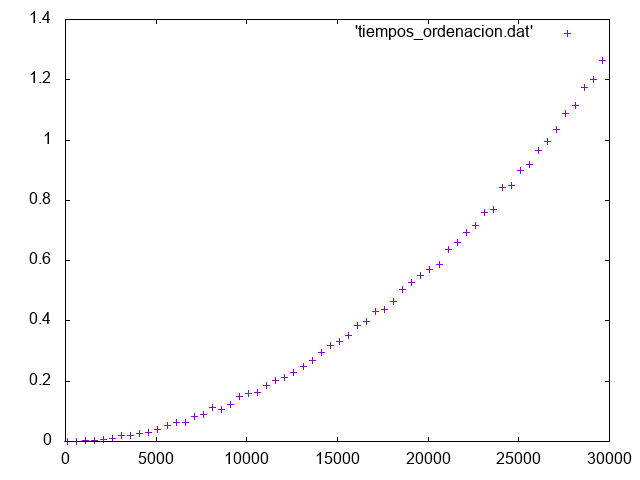
\includegraphics[width=0.8\textwidth]{ejer1/grafica.png}
	\end{figure}


\clearpage
\section{Ejercicio 2 : Ajuste en la ordenación de la burbuja}
Replique el experimento de ajuste por regresión a los resultados obtenidos en el ejercicio 1 que calculaba la eficiencia del algoritmo de ordenación de la burbuja. Para ello considere que f(x) es de la forma ax2+bx+c
\vspace{10mm}

\begin{lstlisting}
gnuplot> f(x) = a*x**2 + b*x + c
gnuplot> fit f(x) 'tiempos_ordenacion.dat' via a,b,c

.....................................................................          

After 12 iterations the fit converged.
final sum of squares of residuals : 0.00377746
rel. change during last iteration : -1.08711e-10

degrees of freedom    (FIT_NDF)                        : 57
rms of residuals      (FIT_STDFIT) = sqrt(WSSR/ndf)    : 0.00814071
variance of residuals (reduced chisquare) = WSSR/ndf   : 6.62712e-05

Final set of parameters            Asymptotic Standard Error
=======================            ==========================
a               = 1.38647e-09      +/- 1.568e-11    (1.131%)
b               = 8.02816e-07      +/- 4.812e-07    (59.94%)
c               = 0.00179818       +/- 0.003092     (171.9%)

correlation matrix of the fit parameters:
                a      b      c      
a               1.000 
b              -0.968  1.000 
c               0.738 -0.861  1.000 
\end{lstlisting}
\vspace{10mm}
	Por tanto mediante gnuplot hemos obtenido las siguiente funci\`on de ejecuci\`on:
	\begin{equation}
		T(n) = \frac{1.39x^2}{10^9} + \frac{8.03x}{10^7} + 0.0018
	\end{equation}

\clearpage
\section{Ejercicio 3 : Problemas de precisión}
Junto con este guión se le ha suministrado un fichero ejercicio\_desc.cpp. En él se ha implementado un algoritmo. Se pide que:
\begin{itemize}
	\item Explique qué hace este algoritmo.
	\item Calcule su eficiencia teórica.
	\item Calcule su eficiencia empírica.
\end{itemize}
Si visualiza la eficiencia empírica debería notar algo anormal. Explíquelo y proponga una solución. Compruebe que su solución es correcta. Una vez resuelto el problema realice la regresioón para ajustar la curva teórica a la empírica.\\
\clearpage


	Se trata de una b\'usqueda binaria. Lo que hace es buscar un valor dentro de un vector subdividiendo el vector en dos partes hasta encontrarlo. Esto solo se puede aplicar a vectores ordenados, ya que el algor\'itmo se basa en que si el valor no esta entre las cotas de un intervalo de valores del vector no puede estar en esas posiciones del vector. \\ \\
	Para calcular la eficiencia te\'orica empezamos fijandonos que el bucle principal se ejecuta $log_2(n)$ veces. Esto es asi porque podemos dividir un n\'umero entre 2 como mucho  $log_2(n)$ veces. Antes de comenzar el bucle se ejecuta 4 OE (la asignaci\'on en linea 1, las comparaciones del inicio del bucle y el AND l\'ogico). Adem\'as dentro del bucle siempre se ejecutaran las 3 OE de la condicion y 3 OE del calculo del \'indice medio. Aplicando la regla de la suma en los bloques condicionales obtenemos que el m\'aximo son 4 OE (acceso a memoria, comparaci\'on, incremento y asignaci\'on) en la segunda sentencia else if. En total en el cuerpo del bucle se ejecutaran como mucho 10 OE. Al terminar el bucle se ejecutan 2 OE m\'as.
	En total tenemos: 
	\begin{equation}
		T(n) = 4 + (3+3+4)log_2(n) + 2 = 6+ 10log_2(n)
	\end{equation} 
	Dividimos por la frecuencia del procesador para hallar el valor en segundos:
	\begin{equation}
		T(n) = \frac{6+10log_2(n)}{1.6*10^9}
	\end{equation}
	
	Mediante gnuplot obtenemos la siguiente eficiencia emp\'irica:
	\begin{figure}[H]
  		\caption{Eficiencia emp\'irica}
  		\centering
  		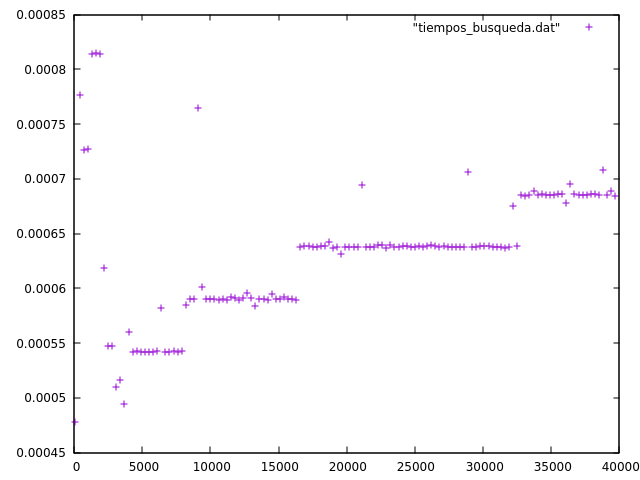
\includegraphics[width=0.8\textwidth]{ejer3/grafica.png}
	\end{figure}
	
	Como el rendimiento de la b\'usqueda binaria es mucho mejor que el de la ordenaci\'on de la burbuja, la ejecuci\'on para valores grandes tarda demasiado tiempo a causa de la ordenaci\'on y no podemos obtener valores fiables para trazar bien la gr\'afica.

\clearpage
\section{Ejercicio 4 :}
Retome el ejercicio de ordenación mediante el algoritmo de la burbuja. Debe modificar el
código que genera los datos de entrada para situarnos en dos escenarios diferentes:
\begin{itemize}
	\item El mejor caso posible. Para este algoritmo, si la entrada es un vector que ya está ordenado el tiempo de cómputo es menor ya que no tiene que intercambiar ningún elemento
	\item El peor caso posible. Si la entrada es un vector ordenado en orden inverso estaremos en la peor situación posible ya que en cada iteración del bucle interno hay que hacer un intercambio.
\end{itemize}
	Calcule la eficiencia empírica en ambos escenarios y compárela con el resultado del ejercicio 1.
\clearpage

Sabemos que en general el tiempo que tarda el procesador en comparar dos enteros no depende de su valor y por tanto nos sirve con crear el vector de entrada m\'as simple. Es decir en el mejor caso el vector [0,1,2,3 ... n] y en el peor caso [n,n-1, ... ,3,2,1,0]. Adem\'as es trivial calcular la eficiencia te\'orica quitando las operaaci\'ones del bloque if obteniendo asi:
	\begin{equation}
			T(n) = 3 + (3+3)(n-1) + \frac{(3+3+)(n-1)(n)}{2} = 3n^2 + 3n -6
	\end{equation}

	Ejecutando la funci\'on con los diferentes tipos de datos obtenemos la siguiente gr\'afica de tiempos de ejecuci\'on de gnuplot:
		\begin{figure}[H]
  		\caption{Diferentes eficiencias}
  		\centering
  		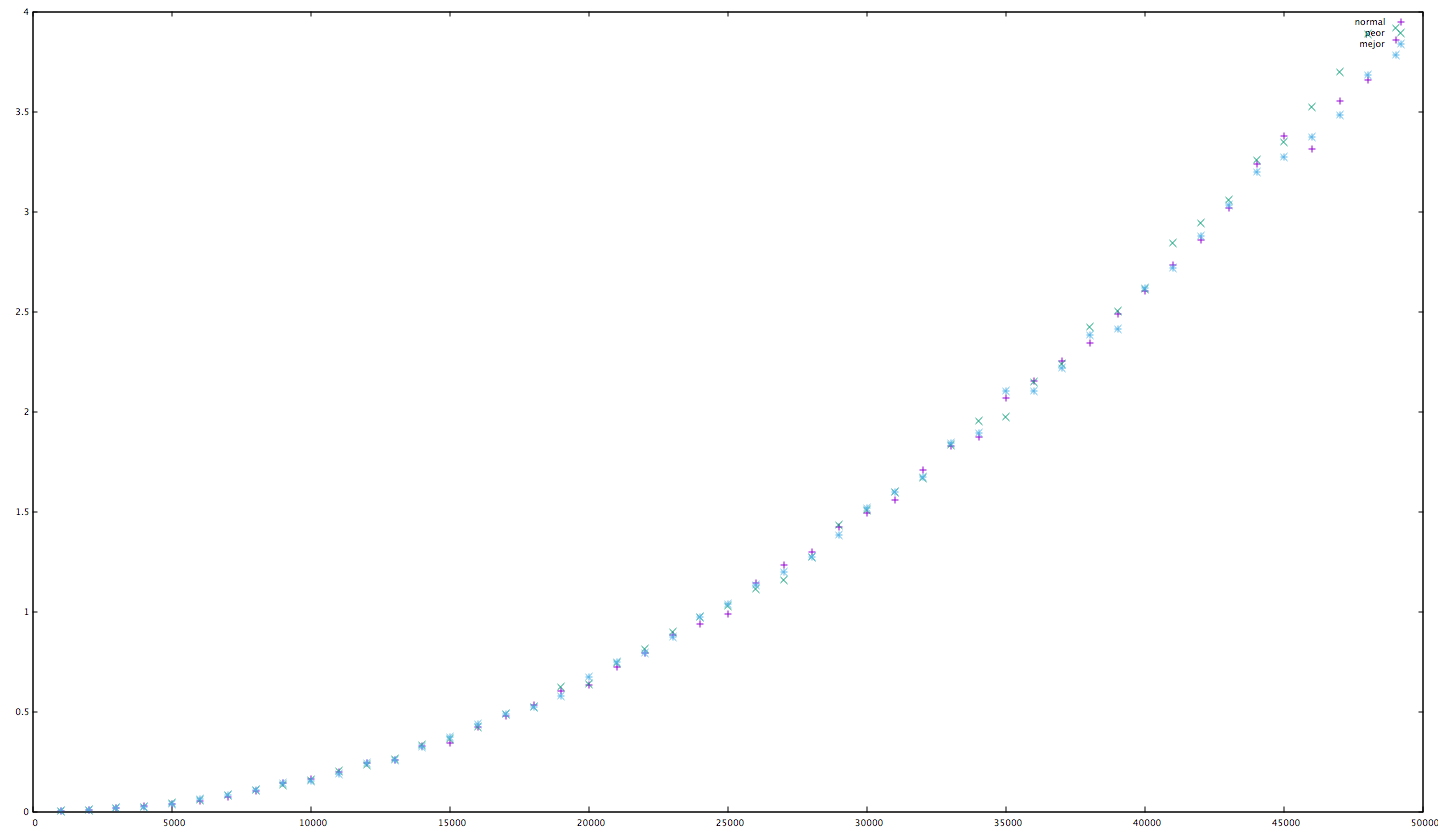
\includegraphics[width=0.8\textwidth]{ejer4/grafica.png}
	\end{figure}
	
	Como vemos, en genera la diferencia suele ser despreciable.


\clearpage
\section{Ejercicio 5 : Dependencia de la implementación}
Considere esta otra implementación del algoritmo de la burbuja:
\begin{lstlisting}
	void ordenar(int *v, int n) {
		bool cambio=true;
		for (int i=0; i<n-1 && cambio; i++) {
			cambio=false;
			for (int j=0; j<n-i-1; j++)
				if (v[j]>v[j+1]) {
					cambio=true;
					int aux = v[j];
					v[j] = v[j+1];
					v[j+1] = aux;
				}
		}
	}
\end{lstlisting}

En ella se ha introducido una variable que permite saber si, en una de las iteraciones del
bucle externo no se ha modificado el vector. Si esto ocurre significa que ya está ordenado
y no hay que continuar.
Considere ahora la situación del mejor caso posible en la que el vector de entrada ya está
ordenado. ¿Cuál sería la eficiencia teórica en ese mejor caso? Muestre la gráfica con la
eficiencia empírica y compruebe si se ajusta a la previsión.
\clearpage
Empecemos calculando la eficiencia teórica:
\begin{itemize}
	\item Línea 2: 1OE (asignación).
	\item Línea 3: 1OE (asignación) + 3OE (resta, comparación,
          operación \&\&) + 1OE (incremento).
	\item Línea 4: 1OE (asignación).
	\item Línea 5: 1OE (asignación) + 3OE (resta*2, comparación) + 1OE (incremento).
	\item Línea 6: 3OE (acceso al elemento [j] y [j+1], comparación).
	\item Línea 7: 1OE (asignación).
	\item Línea 8: 2OE (acceso al elemento [j], asignación).
	\item Línea 9: 3OE (acceso al elemento [j] y [j+1], asignación).
	\item Línea 10: 2OE (acceso al elemento [j+1], asignación).
\end{itemize}
Obtenemos el siguiente tiempo de ejecución en el mejor de los casos
(con el número de línea entre paréntesis):
\begin{align*}
  T(n)= 1OE(2) + 4OE&(3) + 1OE(4) + 4OE(5) + (( 3OE(6) + 1OE(5) +
  3OE(5) )*(n-1))\\& + 1OE(3) + 3OE(3) = 14+7n-7 = 7n+7
\end{align*}
La gráfica obtenida con gnuplot es la siguiente
\begin{figure}[H]
  \caption{Eficiencia en el mejor caso}
  \centering
  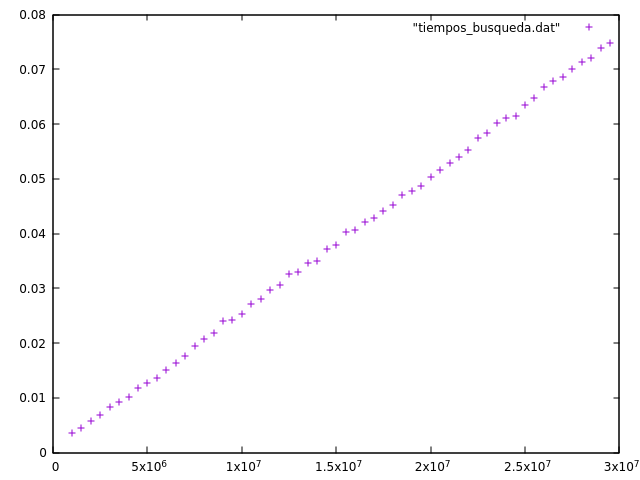
\includegraphics[width=0.8\textwidth]{ejer5/grafica.png}
\end{figure}
Como podemos ver si se ajuta a la teórica pues la mayoría de valores
de la gráfica se agrupan formando una recta.
\clearpage
\section{Ejercicio 6 : Influencia del proceso de compilación}
Retome el ejercicio de ordenación mediante el algoritmo de la burbuja. Ahora replique
dicho ejercicio pero previamente deberá compilar el programa indicándole al compilador
que optimice el código. Esto se consigue así:
\begin{verbatim}
g++ -O3 ordenacion.cpp -o ordenacion\_optimizado
\end{verbatim}
Compare las curvas de eficiencia empírica para ver cómo mejora esto la eficiencia del programa.
\clearpage
La diferencia en eficiencia cuando se utiliza la opcion -O3 se puede ver claramente en la siguiente gráfica donde se han representado los datos obtenidos en ambos casos: 
\begin{figure}[H]
  \centering
  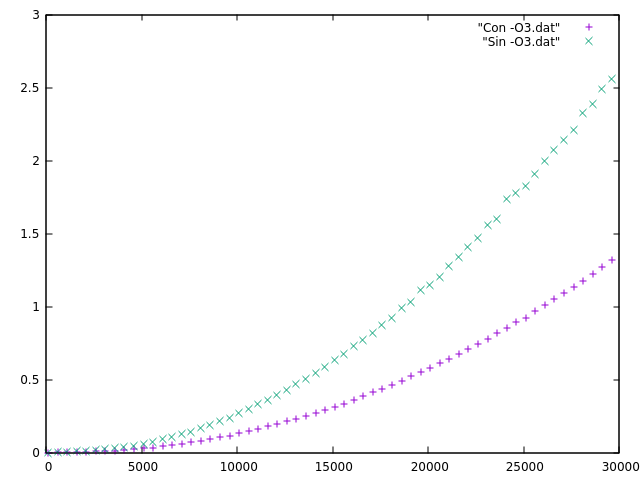
\includegraphics[width=0.8\textwidth]{comparacion.png}
\end{figure}
Podemos ver claramente como el tiempo de ejecución se reduce considerablemente.
\end{document}
